\chapter{Predict and optimize}


\section{Approaches}


\subsection{Prediction focused learning}

\begin{description}
    \item[Prediction focused learning] \marginnote{Prediction focused learning}
        Inference method that solves an optimization problem by using inputs predicted by an estimator. More specifically, there are two steps:
        \begin{descriptionlist}
            \item[Predict] 
                Train a predictor for the parameters of the problem. The optimal predictor $h$ has the following parameters:
                \[ \theta^* = \arg\min_\theta \left\{ \mathbb{E}_{(x, y) \sim P(X, Y)}[\mathcal{L}(y, \hat{y})] \mid \hat{y} = h(x, \theta) \right\} \]

            \item[Optimize] 
                Solve an optimization problem with the estimated parameters as input:
                \[ z^*(y) = \arg\min_\vec{z} \left\{ f(\vec{z}, y) \mid \vec{z} \in F \right\} \]
                where $\vec{z}$ is the decision vector, $f$ is the cost function, $F$ is the feasible space, and $y$ is the output of the predictor $h$.
        \end{descriptionlist}

        Therefore, during inference, the following is computed:
        \[ z^*(h(x; \theta)) = z^*(\hat{y}) \]

        \begin{figure}[H]
            \centering
            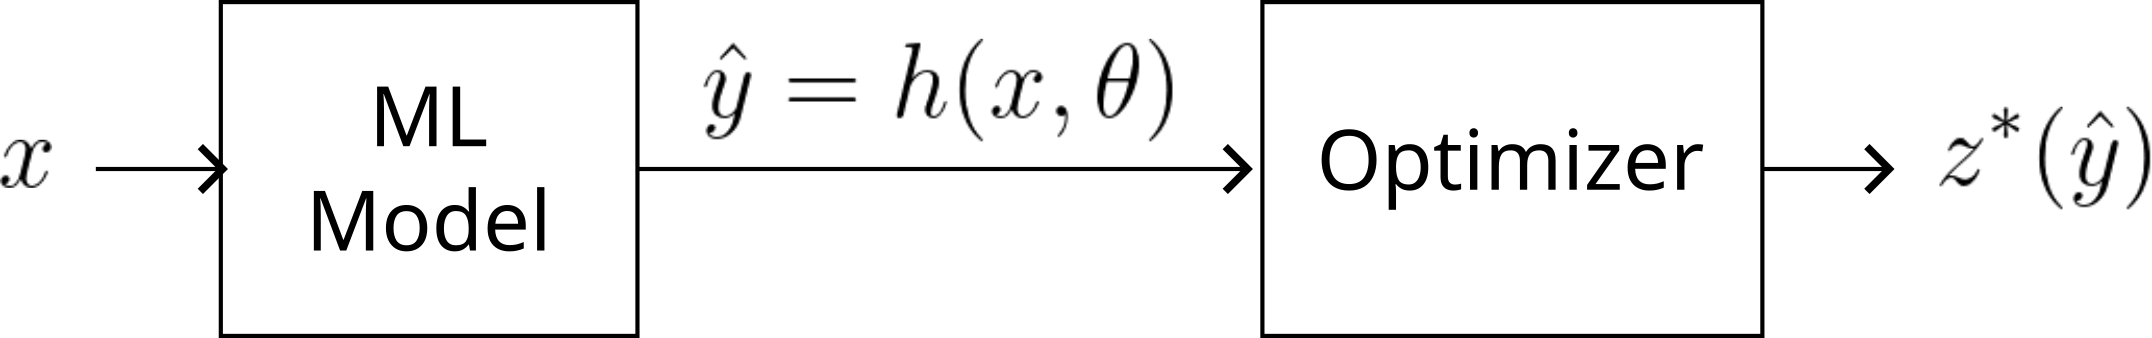
\includegraphics[width=0.5\linewidth]{./img/dfl_setup.png}
        \end{figure}

        \begin{remark}
            This approach is asymptotically correct. The perfect predictor allows to reach the optimal result.
        \end{remark}

        \begin{remark}
            The predictor should be trained for minimal decision cost (instead of maximal accuracy) so that the optimizer can make the correct choice.
        \end{remark}

        \begin{example}
            Consider the problem:
            \[ \arg\min_{z} \{y_0 z_0 + y_1 z_1 \mid z_0 + z_1 = 1, z \in \{0, 1\}^2\} \]
            with some ground-truth $y_0$ and $y_1$.
            Assume that the predictor can only learn a model of form:
            \[ \hat{y}_0 = \theta^2x \qquad \hat{y}_1 = 0.5 \cdot \theta \]
            By maximizing accuracy, the following predictions are obtained:
            \begin{figure}[H]
                \centering
                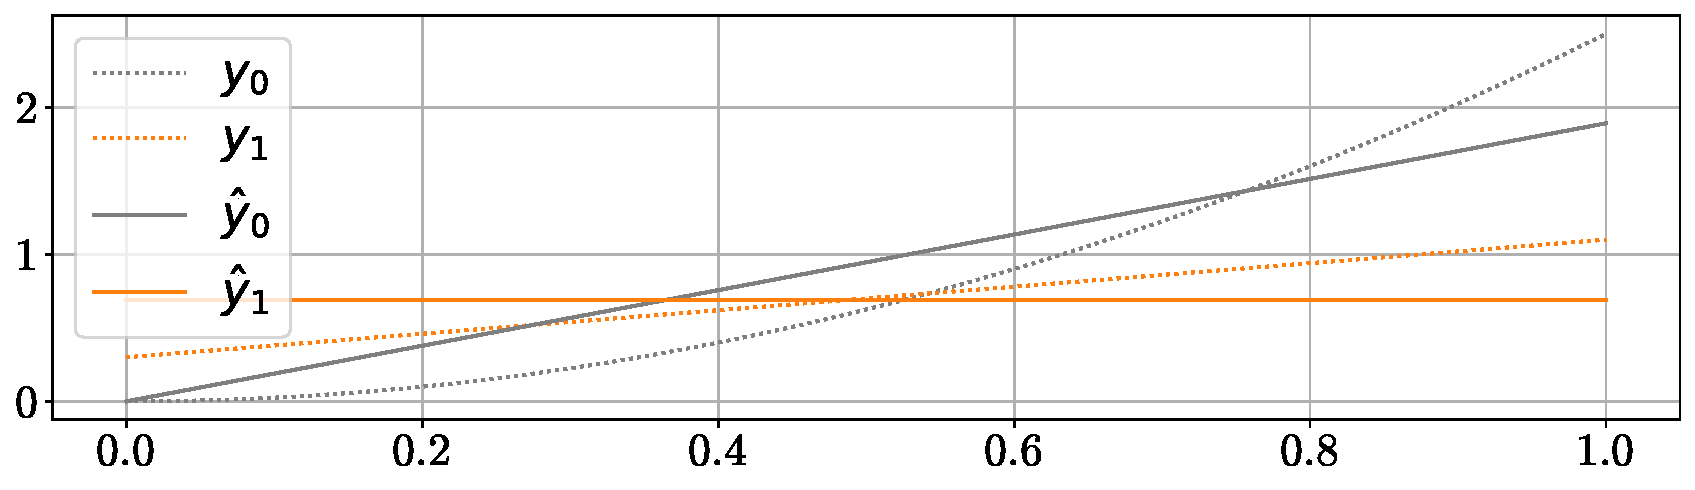
\includegraphics[width=0.7\linewidth]{./img/_pfl_example1.pdf}
            \end{figure}
            The intersection point is important for optimization. In this case, predictions are not ideal. Instead, by minimizing decision cost, the following predictions are made:
            \begin{figure}[H]
                \centering
                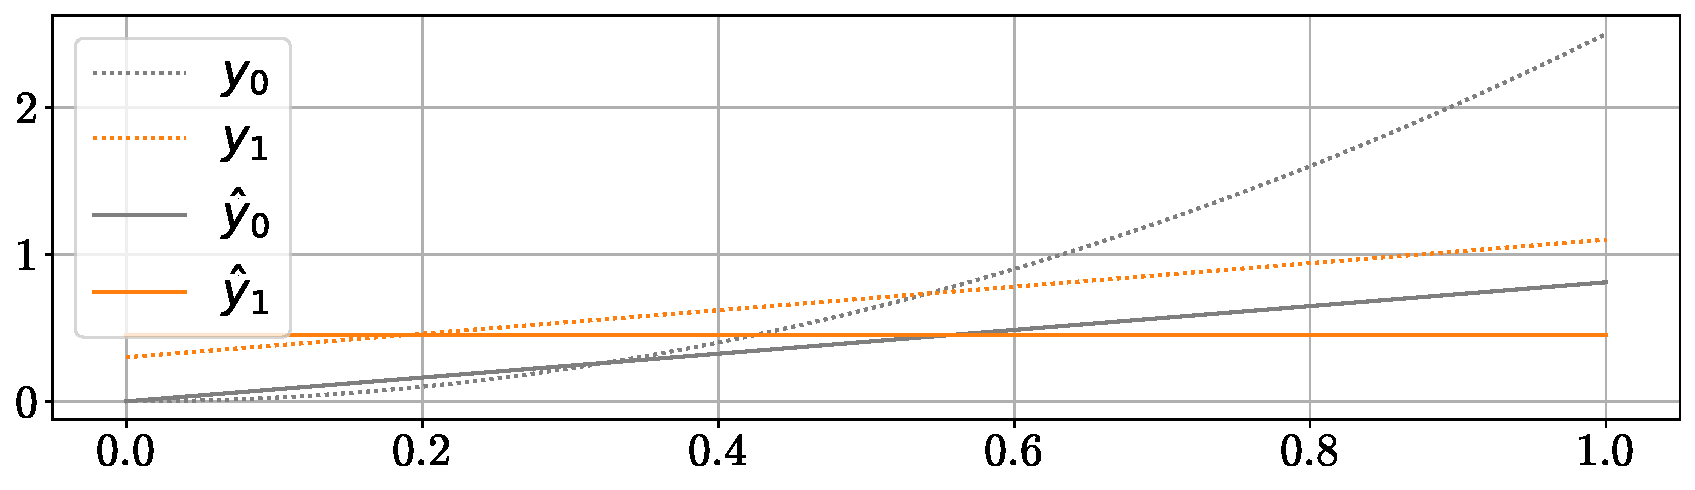
\includegraphics[width=0.7\linewidth]{./img/_pfl_example2.pdf}
            \end{figure}
        \end{example}
\end{description}


\subsection{Decision focused learning}

\begin{description}
    \item[Decision focused learning (DFL)] \marginnote{Decision focused learning (DFL)}
        PFD where linear cost functions are assumed. The optimization problem is therefore:
        \[ z^*(y) = \arg\min_z \{ y^Tz \mid z \in F \} \]
        where $y$ cannot be measured but depends on some observable $x$ (i.e., $X, Y \sim P(X, Y)$).

        The training problem of the predictor aims to minimize the decision cost and is defined as:
        \[ 
            \theta^* = \arg\min_\theta = \left\{ \mathbb{E}_{(x, y) \sim P(X,Y)} \left[ \texttt{regret}(y, \hat{y}) \mid \hat{y} = h(x, \theta) \right] \right\} 
        \]

        \begin{description}
            \item[Regret] \marginnote{Regret}
                Measures the difference between the solution obtained using the predictor and the perfect solution. It is defined as:
                \[ \texttt{regret}(y, \hat{y}) = y^T z^*(\hat{y}) - y^T z^*(y) \]
                where:
                \begin{itemize}
                    \item $z^*(y)$ is the best solution with access to the ground-truth (i.e., an oracle).
                    \item $z^*(\hat{y})$ is the solution computed with the estimated parameters.
                \end{itemize}

                \begin{remark}
                    Optimizing regret is equivalent to optimizing the cost function, but regret is lower-bounded at $0$.
                \end{remark}

                \begin{remark}
                    Regret is non-differentiable in many points and, when it is, its gradient is not informative. In practice, a surrogate for regret is used instead.
                \end{remark}

                \begin{example}
                    Consider a collection of normally distributed data $(x, y)$:
                    \begin{figure}[H]
                        \centering
                        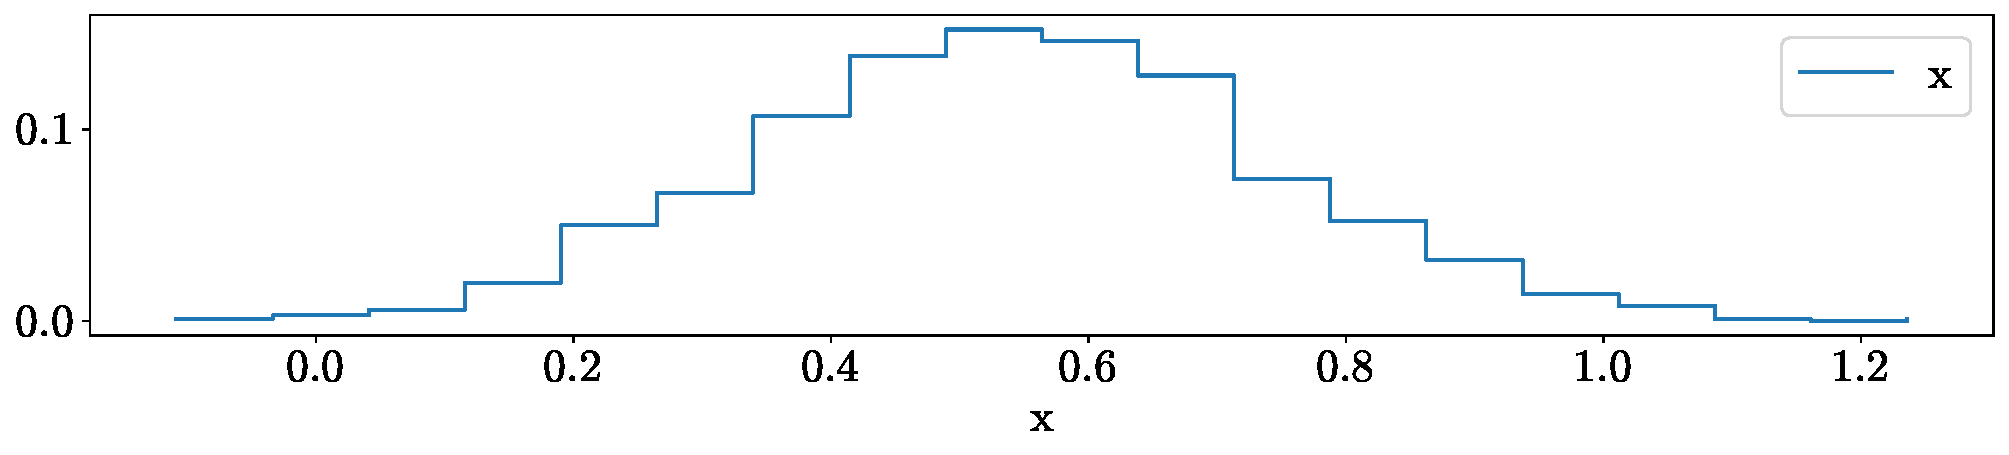
\includegraphics[width=0.75\linewidth]{./img/_dfl_regret_example1.pdf}
                    \end{figure}

                    The regret landscape for varying parameter $\theta$ is:
                    \begin{figure}[H]
                        \centering
                        \begin{subfigure}{0.49\linewidth}
                            \centering
                            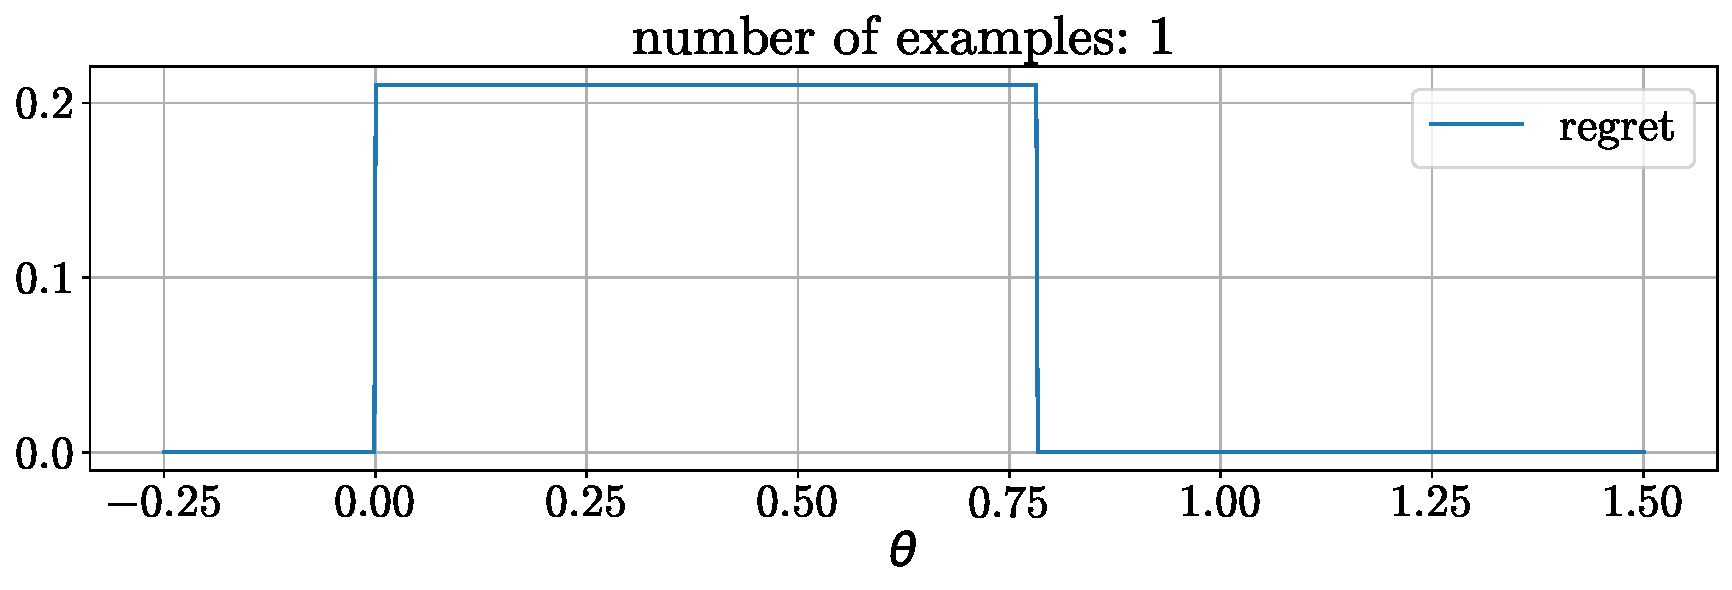
\includegraphics[width=\linewidth]{./img/_dfl_regret_example2.pdf}
                            \caption{Regret for a single sample}
                        \end{subfigure}
                        \begin{subfigure}{0.49\linewidth}
                            \centering
                            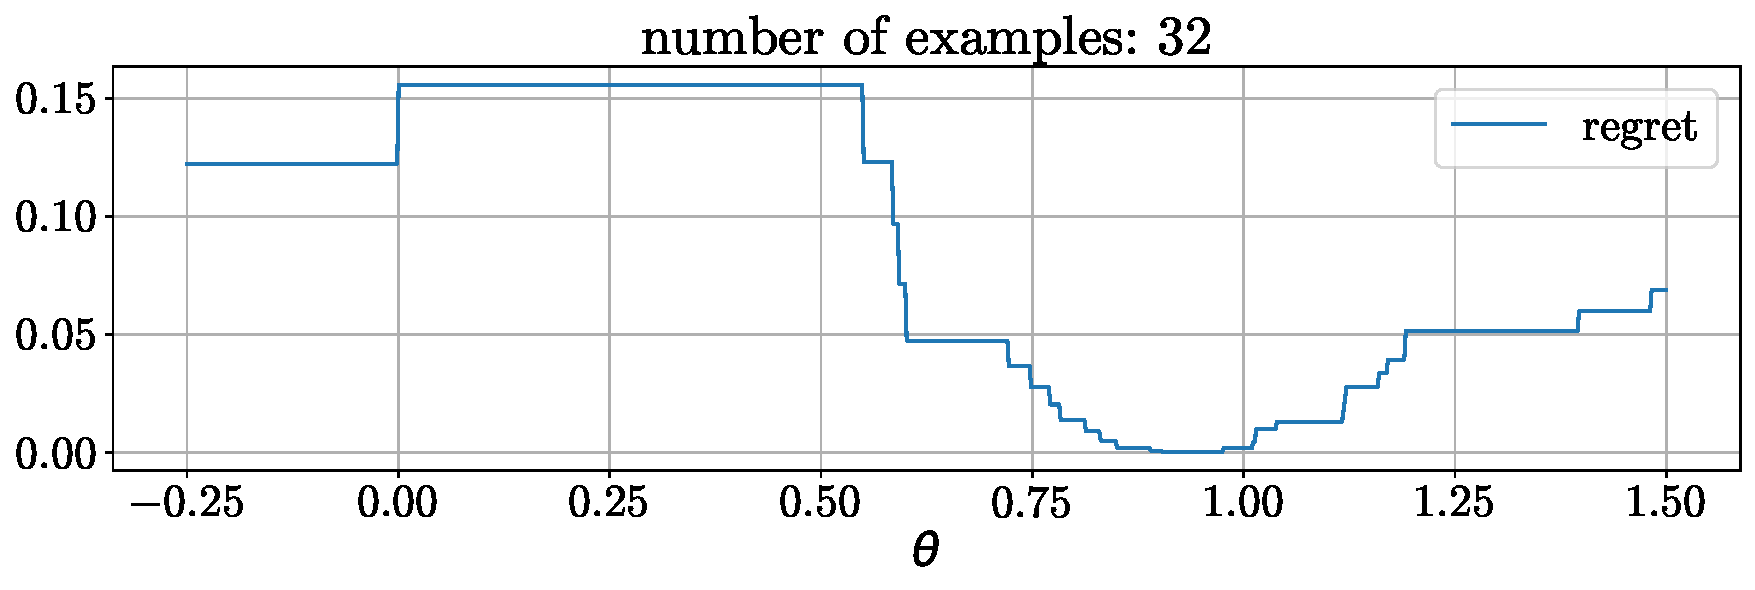
\includegraphics[width=\linewidth]{./img/_dfl_regret_example3.pdf}
                            \caption{Regret for a batch}
                        \end{subfigure}
                    \end{figure}
                \end{example}

            \item[Self-contrastive loss] \marginnote{Self-contrastive loss}
                Surrogate for regret defined as:
                \[ \hat{y}^T z^*(y) - \hat{y}^T z^*(\hat{y}) \] 
                The idea is that a good prediction vector $\hat{y}$ should make the optimal cost $\hat{y}^T z^*(y)$ not worse than the cost of the estimated one $\hat{y}^T z^*(\hat{y})$.

                \begin{remark}
                    By differentiating over $\hat{y}$, the result is a subgradient (i.e., coefficient used to compute a non-defined gradient) and it is computed as:
                    \[ \nabla(\hat{y}^T z^*(y) - \hat{y}^T z^*(\hat{y})) = z^*(y) - z^*(\hat{y}) \]
                \end{remark}

                \begin{remark}
                    Self-contrastive loss creates spurious minima (i.e., false minima that are not in the regret) as a trivial solution is to predict $\hat{y} = 0$.
                \end{remark}

                \begin{example}
                    The self-contrastive loss using the same data as before is:
                    \begin{figure}[H]
                        \centering
                        \begin{subfigure}{0.49\linewidth}
                            \centering
                            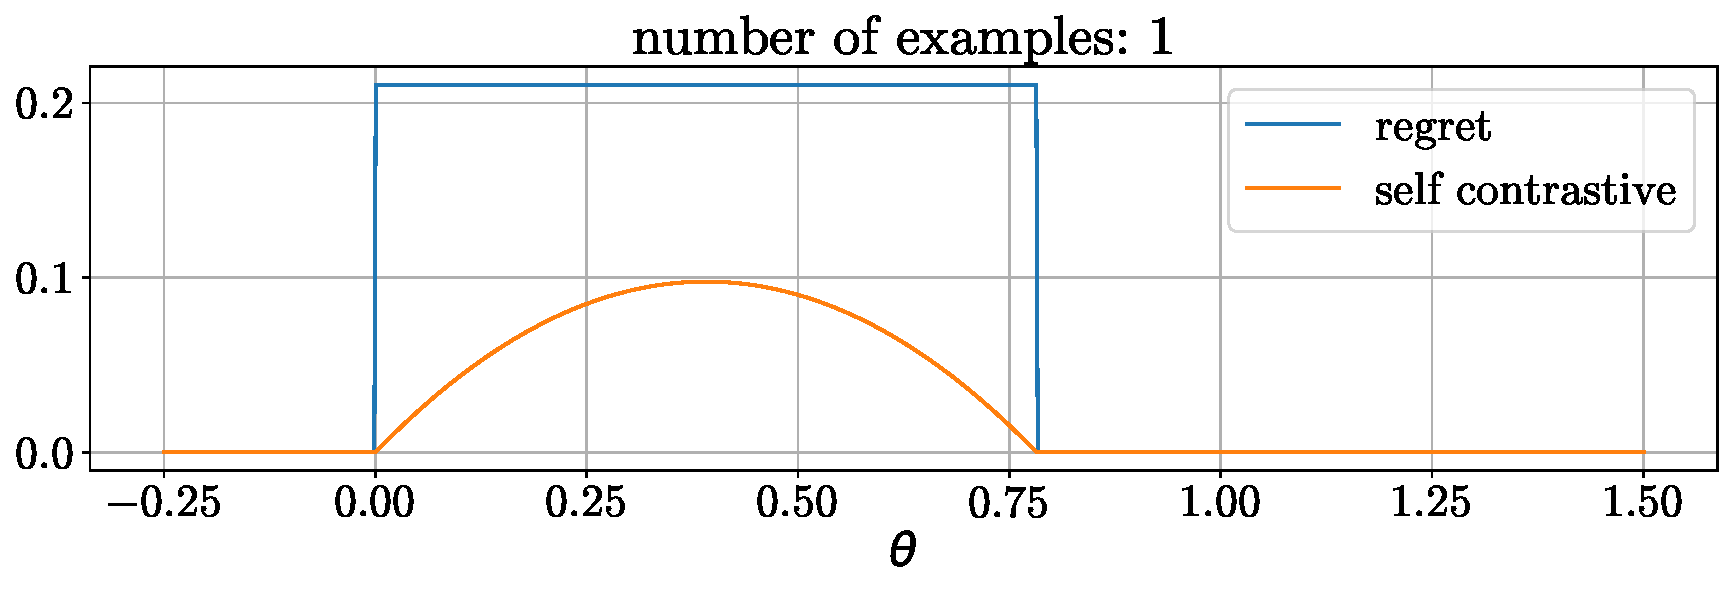
\includegraphics[width=\linewidth]{./img/_dfl_self_contrastive_example1.pdf}
                            \caption{Self-contrastive loss for a single sample}
                        \end{subfigure}
                        \begin{subfigure}{0.49\linewidth}
                            \centering
                            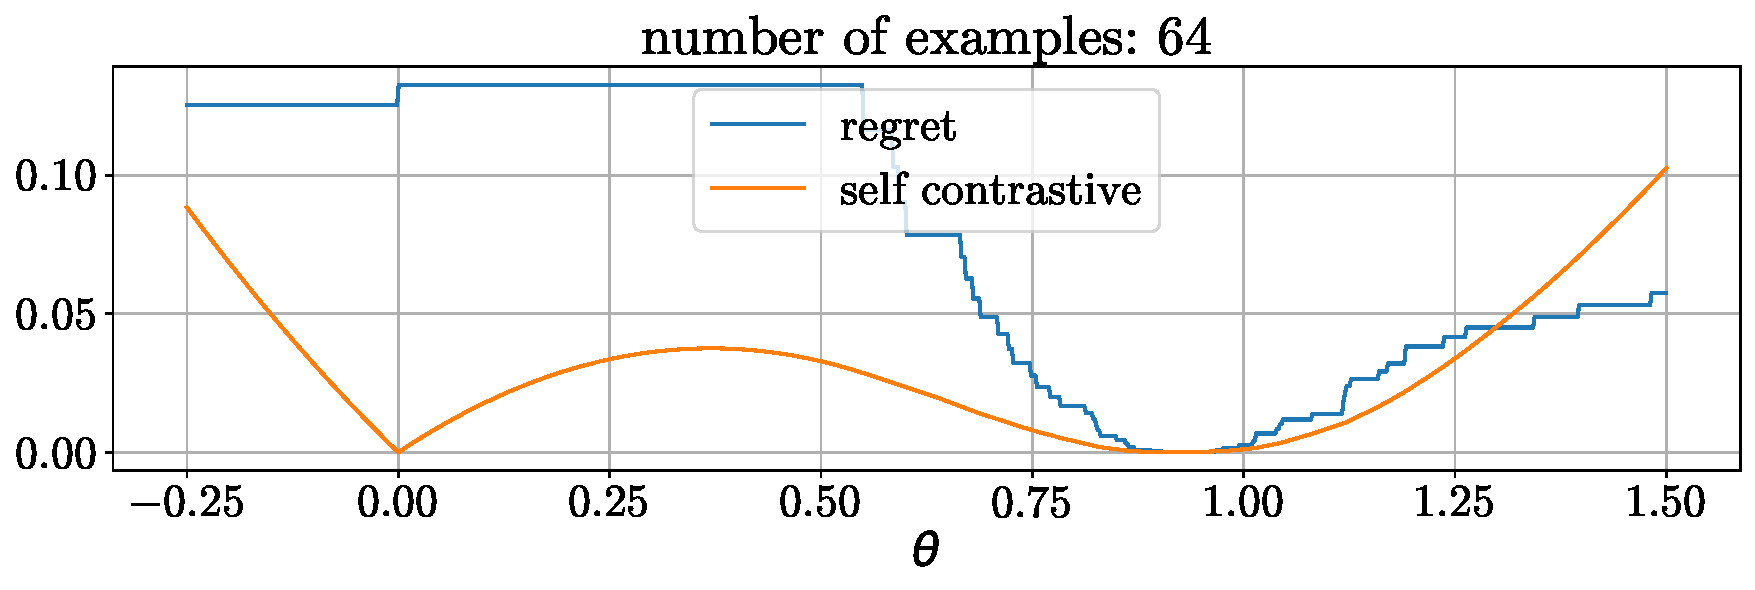
\includegraphics[width=\linewidth]{./img/_dfl_self_contrastive_example2.pdf}
                            \caption{Self-contrastive loss for a batch}
                        \end{subfigure}
                    \end{figure}
                \end{example}

            \item[SPO+ loss] \marginnote{SPO+ loss}
                Surrogate for regret defined as a perturbed version of the self-contrastive loss:
                \[ 
                    \texttt{spo+}(y, \hat{y}) = \hat{y}^T_\text{spo} z^*(y) - \hat{y}^T_\text{spo} z^*(\hat{y}_\text{spo}) \qquad \text{with } \hat{y}_\text{spo} = 2 \hat{y} - y
                \]

                \begin{remark}
                    With many samples, the spurious minima tend to cancel out.
                \end{remark}

                \begin{example}
                    The SPO+ loss using the same data as before is:
                    \begin{figure}[H]
                        \centering
                        \begin{subfigure}{0.49\linewidth}
                            \centering
                            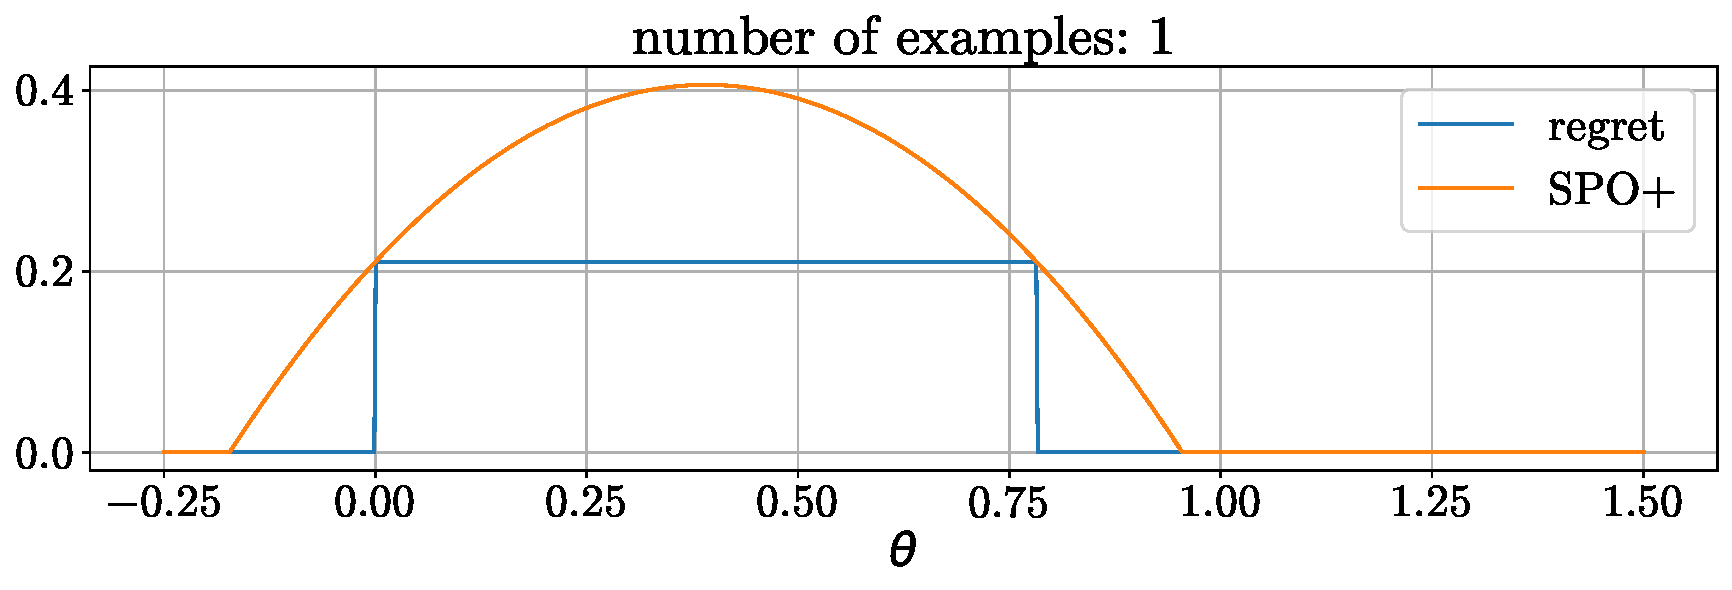
\includegraphics[width=\linewidth]{./img/_dfl_spop_example1.pdf}
                            \caption{SPO+ for a single sample}
                        \end{subfigure}
                        \begin{subfigure}{0.49\linewidth}
                            \centering
                            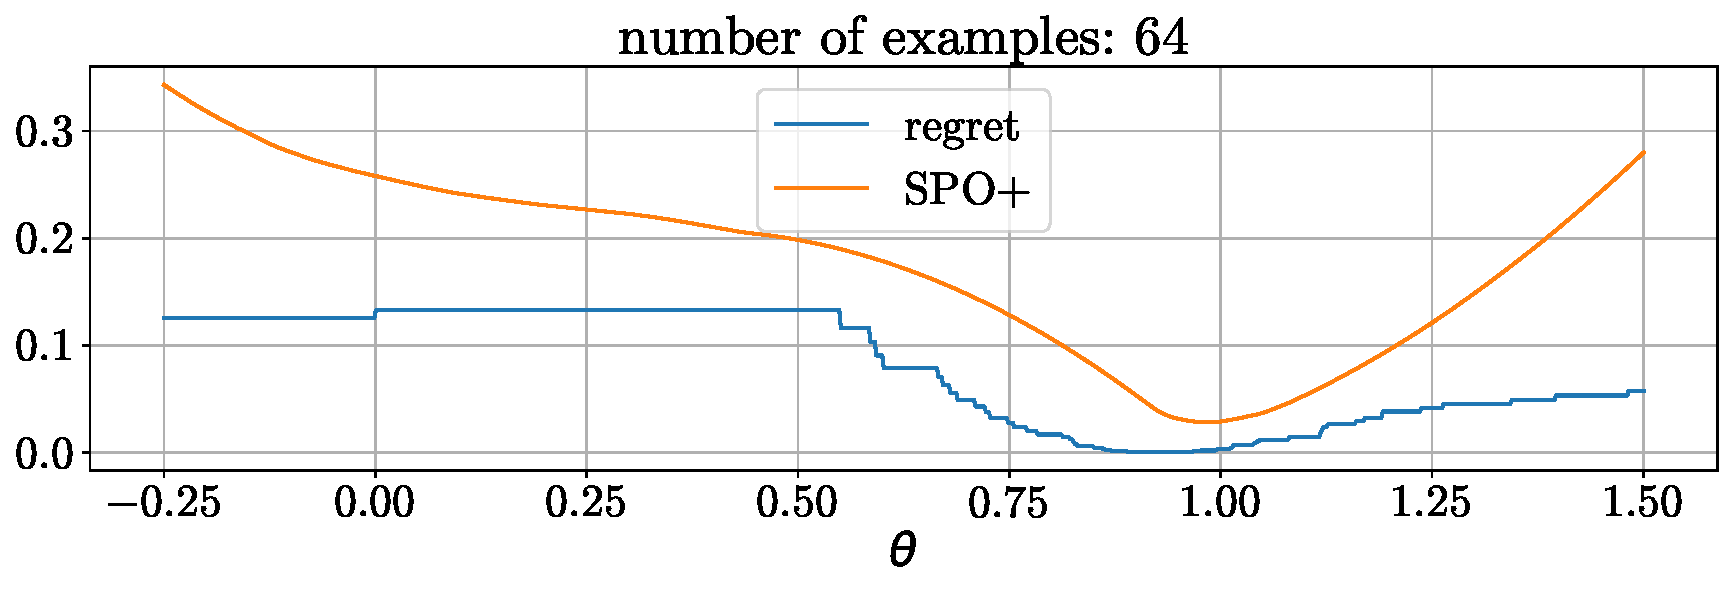
\includegraphics[width=\linewidth]{./img/_dfl_spop_example2.pdf}
                            \caption{SPO+ for a batch}
                        \end{subfigure}
                    \end{figure}
                \end{example}
        \end{description}

        \begin{remark}
            DLF are slow to train as each iteration requires to solve an optimization problem.
        \end{remark}

        \begin{description}
            \item[DLF training speed-up] \phantom{}
            \begin{description}
                \item[Warm start] 
                    Initialize a DFL network with PFL weights.
    
                \item[Solution caching] 
                    Assuming that the feasible space is constant, caching can be done as follows:
                    \begin{enumerate}
                        \item Initialize the cache $\mathcal{S}$ with the true optimal solutions $z^*(y_i)$.
                        \item When it is required to compute $z^*(\hat{y})$:
                        \begin{itemize}
                            \item With probability $p$, invoke the solver and compute the real solution. The newly computed value is cached.
                            \item With probability $p-1$, do a cache lookup as:
                            \[ \hat{z}^*(\hat{y}) = \arg\min_z \{ f(z) \mid z \in \mathcal{S} \} \]
                        \end{itemize}
                    \end{enumerate}
            \end{description}
        \end{description}
\end{description}

\begin{remark}
    PFL with more complex networks allows reaching comparable performance to DLF.
\end{remark}

\begin{remark}
    PFL cannot make perfect predictions in presence of uncertainty.
\end{remark}


\subsection{Two-stage stochastic optimization}

\begin{description}
    \item[Two-stage stochastic optimization (2s-SOP)] \marginnote{Two-stage stochastic optimization (2s-SOP)}
        Optimization performed in two steps:
        \begin{descriptionlist}
            \item[First-stage decisions] Make an initial set of decisions from the current state.
            \item[Recourse actions] Observe uncertainty and make a second set of decisions.
        \end{descriptionlist}

        Formally, 2s-SOP is defined as:
        \[ \arg\min_z \left\{ f(z) + \underset{y \sim P(Y|x)}{\mathbb{E}}\left[ \min_{z''} r(z'', z, y) \right] \mid z \in F, z'' \in F''(z, y) \right\} \]
        where:
        \begin{itemize}
            \item $Y$ models the uncertainty information.
            \item $z$ and $F$ are the first-stage decisions and their feasible space, respectively.
            \item $z''$ and $F''(z, y)$ are the recourse actions and their feasible space, respectively.
            \item $f$ is the immediate cost function of the first-stage decisions.
            \item $r$ is the cost of the recourse actions.
        \end{itemize}

        \begin{example}
            Consider the case of supply planning where we buy from primary suppliers first and then from another sources (for a higher price) in case the primary suppliers are unable to satisfy the request.

            In 2s-SOP, the problem can be formulated as:
            \[ 
                \begin{gathered}
                    \arg\min_z c^Tz + \underset{y \sim P(Y|x)}{\mathbb{E}}\left[ \min_{z''} c''z'' \right] \\
                    \begin{aligned}
                        \text{subject to } &y^Tz + z'' \geq y_\text{min} \\
                        &z \in \{ 0, 1 \}^n, z'' \in \mathbb{N}_0
                    \end{aligned}
                \end{gathered}
            \]
            where:
            \begin{itemize}
                \item $z_j = 1$ iff we choose the $j$-th supplier.
                \item $c_j$ is the cost of the $j$-th supplier.
                \item $y_j$ is the yield of the $j$-th supplier and represents the uncertainty.
                \item $y_\text{min}$ is the minimum required yield.
                \item $z''$ is the amount we buy at cost $c''$.
            \end{itemize}
        \end{example}


    \item[2s-SOP without uncertainty] \marginnote{2s-SOP without uncertainty}
        Solve a 2s-SOP problem by ignoring the uncertainty part (i.e., $\mathbb{E}_{y \sim P(Y|x)}\left[ \min_{z''} r(z'', z, y) \right]$).


    \item[Scenario based 2s-SOP] \marginnote{Scenario based 2s-SOP}
        Sample a finite set of scenarios from $P(Y | x)$ and define different recourse action variables for each scenario.

        \begin{example}
            For supply planning, the problem becomes:
            \[ 
                \begin{gathered}
                    \arg\min_z c^Tz + \frac{1}{N} c'' z_{k}'' \\
                    \begin{aligned}
                        \text{subject to } &y^Tz + z_{k}'' \geq y_\text{min} & \forall k = 1, \dots, N \\
                        &z \in \{ 0, 1 \}^n \\
                        &z_k'' \in \mathbb{N}_0 & \forall k = 1, \dots, N
                    \end{aligned}
                \end{gathered}
            \]
        \end{example}

        \begin{remark}
            This approach is effective but it is computationally expensive.
        \end{remark}


    \item[DFL for 2s-SOP] \marginnote{DFL for 2s-SOP}
        Consider the formulation of DFL problems:
        \[ 
            \theta^* = \arg\min_\theta \left\{\underset{(x, y) \sim P(X, Y)}{\mathbb{E}}\left[ \texttt{regret}(y, \hat{y}) \right] \mid \hat{y} = h(x; \theta) \right\} 
        \]
        To change this formulation to make it closer to 2s-SOP, we can:
        \begin{itemize}
            \item Use a generic cost function $g$ instead of the regret (the minimization objective does not change).
            \item Focus on a single observable $x$ (i.e., a single instance of the problem).
            \item Add the constraint $z^*(\hat{y}) \in F$ (which is always satisfied by construction).
        \end{itemize}
        The formulation becomes:
        \[ 
            \theta^* = \arg\min_\theta \left\{\underset{y \sim P(Y|x)}{\mathbb{E}}\left[ g(z^*(\hat{y}), y) \right] \mid \hat{y} = h(x; \theta), z^*(\hat{y}) \in F \right\} 
        \]
        By specifically choosing $g$ as:
        \[ g(z, y) = \min_{z''} \left\{ f(z) + r(z'', z, y) \mid z'' \in F''(z, y) \right\} \]
        The final problem can be formulated as:
        \[ 
            \begin{gathered}
                \arg\min_\theta f(z^*(\hat{y})) + \underset{y \sim P(Y|x)}{\mathbb{E}}\left[ \min_{z''} r(z'', z^*(\hat{y}), y) \right]  \\ 
                \begin{aligned}
                    \text{subject to } &\hat{y} = h(x; \theta) \\ 
                    &z^*(\hat{y}) \in F \\
                    &z'' \in F''(z, y) \\
                \end{aligned}
            \end{gathered}
        \]
        Which is close to 2s-SOP formulated as a training problem on the parameters $\theta$ that is considering a single example (i.e., $x$ is fixed).

        \begin{remark}
            With this formulation, at inference time, only a single scenario is needed to obtain good results (i.e., more scalability). Moreover, existing solvers can be used without modifications.
        \end{remark}

        \begin{example}
            In the supply planning case, the problem becomes:
            \[
                \begin{gathered}
                    z^*(y) = \arg\min_z \left\{ \min_{z''} c^Tz + c''z_k'' \right\} \\
                    \begin{aligned}
                        \text{subject to } &y^Tz + z_k'' \geq y_\text{min} \\
                        &z \in \{ 0, 1 \}^n \\
                        &z_k'' \in \mathbb{N}_0
                    \end{aligned}
                \end{gathered}
            \]
            Note that the expected value is not needed as we are considering a single scenario.
        \end{example}

        \begin{description}
            \item[Stochastic smoothing] \marginnote{Stochastic smoothing}
                Apply a Gaussian kernel on the loss function to smooth it and make it differentiable.

                Formally, the loss becomes:
                \[ 
                    \tilde{\mathcal{L}}_\text{DFL}(\theta) =
                    \underset{\substack{(x, y) \sim P(X, Y)\\\hat{y} \sim \mathcal{N}(h(x; \theta))}}{\mathbb{E}}[ \texttt{regret}(y, \hat{y}) ]
                \]

                \begin{remark}
                    Using more samples allows achieving better smoothing. Larger $\sigma$ allows removing flat regions but shifts the optimum.
                \end{remark}

                \begin{figure}[H]
                    \centering
                    \begin{subfigure}{0.7\linewidth}
                        \centering
                        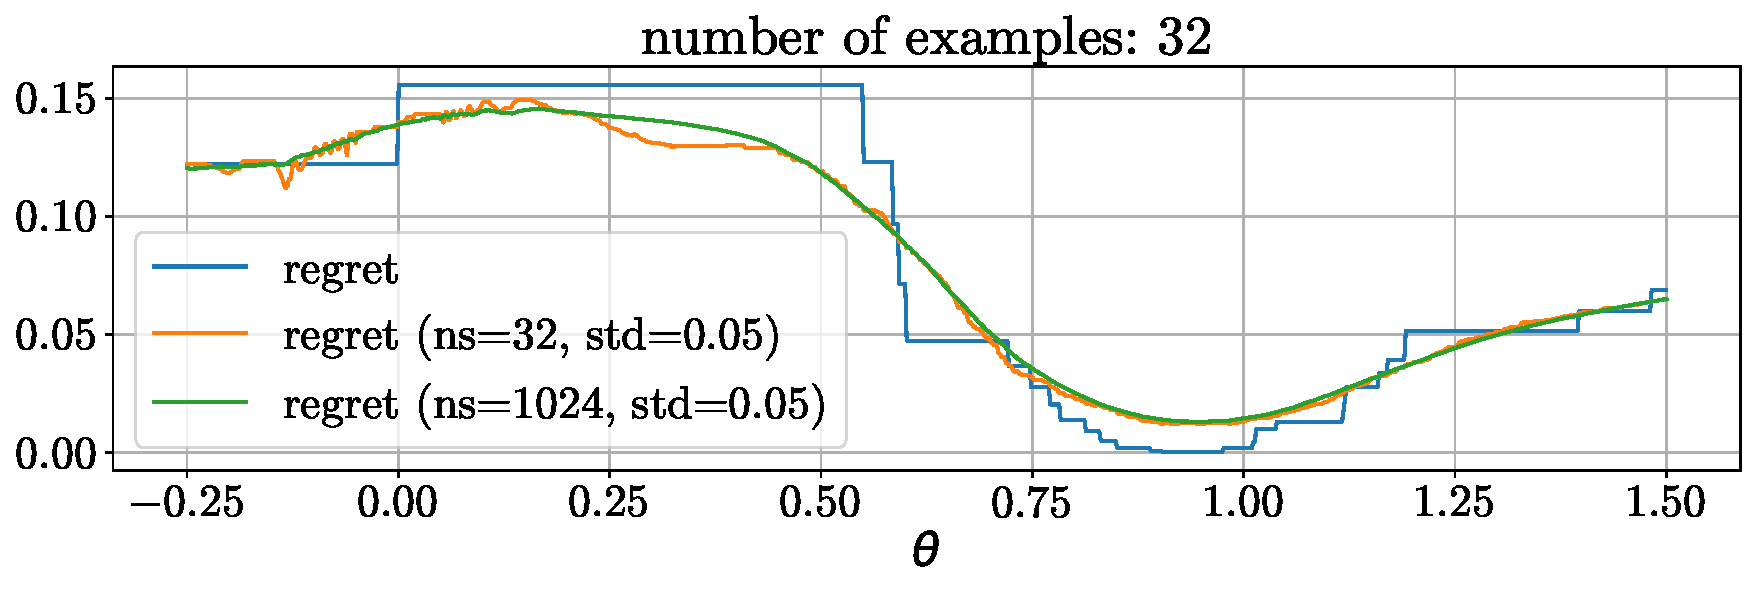
\includegraphics[width=\linewidth]{./img/_dfl_stochastic_smoothing1.pdf}
                    \end{subfigure}
                    \centering
                    \begin{subfigure}{0.7\linewidth}
                        \centering
                        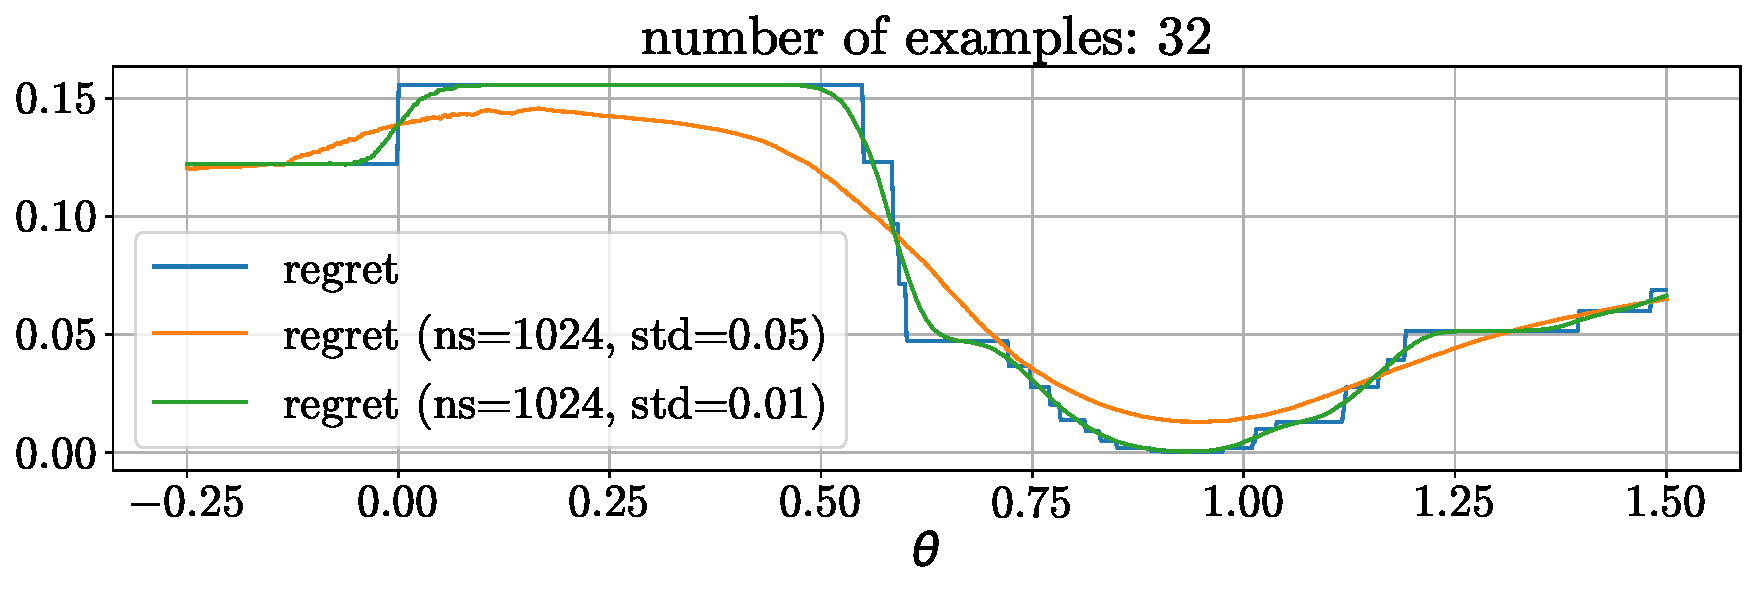
\includegraphics[width=\linewidth]{./img/_dfl_stochastic_smoothing2.pdf}
                    \end{subfigure}
                \end{figure}
        \end{description}
\end{description}